\section{Exercise one}

Consider the process described by the expression: 
\[y(t)=e(t)+5e(t-1)\qquad e(t\sim WN(1,1))\]
The expected value of the process $y(t)$ is six. 

Find the unbiased process. 

\subsection{Solution}
The given system can be represented as: 
\begin{figure}[H]
    \centering
    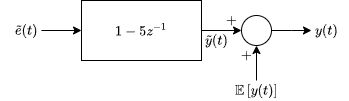
\includegraphics[width=0.5\linewidth]{images/bias.png}
\end{figure}
In the block diagram we have defined: 
\[\begin{cases}
    \tilde{y}(t)=y(t)-m_y \\
    \tilde{e}(t)=e(t)-m_e 
\end{cases}\rightarrow \begin{cases}
    \tilde{y}(t)=y(t)-6 \\
    \tilde{e}(t)=e(t)-1 
\end{cases}\]
The process $y(t)$ is composed by: 
\[y(t)=\tilde{y}(t)+6=\tilde{e}(t)\left( 1+5z^{-1} \right)+6=\left(e(t)-1\right)\left( 1+5z^{-1} \right)+6=e(t)+5e(t-1)\]
The unbiased process is: 
\[\tilde{y}(t)=\tilde{e}(t)+5\tilde{e}(t-1)\]

The unbiased process is not in canonical form, so we must use an all-pass filter: 
\[\tilde{y}(t)=\dfrac{1+\frac{1}{5}z^{-1}}{1}\dfrac{1+5z^{-1}}{1+\frac{1}{5}z^{-1}1}\tilde{e}(t)\]











